% SPIE Defense + Security 2026
% Paper ID: 14030-26
% Track: DS112 - Machine Learning from Challenging Data
%
% Title: Predictive Target Pursuit for Autonomous UAVs using RF-DETR
%        with Depth-Aware State Estimation and Physics-Informed
%        Trajectory Prediction
%
% Use SPIE Proceedings template: \documentclass[]{spieproc}
% For now, using article class as scaffold. Switch to spieproc for submission.

\documentclass[11pt,letterpaper]{article}

% --- Page layout (approximate SPIE format) ---
\usepackage[margin=1in]{geometry}

% --- Fonts ---
\usepackage{times}
\usepackage[T1]{fontenc}

% --- Math ---
\usepackage{amsmath}
\usepackage{amssymb}

% --- Graphics ---
\usepackage{graphicx}
\graphicspath{{figures/}}
\usepackage{subcaption}

% --- Tables ---
\usepackage{booktabs}
\usepackage{array}
\usepackage{multirow}

% --- Units ---
\usepackage{siunitx}
\sisetup{per-mode=symbol}

% --- Code / topic names ---
\usepackage{listings}
\lstset{basicstyle=\ttfamily\small, breaklines=true}

% --- Citations ---
\usepackage[numbers,sort&compress]{natbib}

% --- Hyperlinks ---
\usepackage{hyperref}
\hypersetup{hidelinks}

% --- Captions ---
\usepackage{caption}
\captionsetup{font=small, labelfont=bf}

% ============================================================================
\begin{document}

\title{Predictive Target Pursuit for Autonomous UAVs using RF-DETR with Depth-Aware State Estimation and Physics-Informed Trajectory Prediction}

\author{
    % Author list TBD - add all team members
    % Embry-Riddle Aeronautical University, Daytona Beach, FL
}

\date{}
\maketitle

% ============================================================================
\begin{abstract}
% TODO: Write after all sections are drafted (Lead owns this)
\end{abstract}

% ============================================================================
\section{Introduction}
\label{sec:intro}
% TODO: Lead + Tracking team (PINN lit review)
% - Motivation: autonomous UAV pursuit in degraded visual conditions
% - Gap: CNN detectors degrade under noise/blur, reactive control fails during dropouts
% - Contribution summary (5 novel elements from roadmap)

% ============================================================================
\section{Related Work}
\label{sec:related}
% TODO: Lead + Tracking team
% - Object detection on embedded platforms (YOLO family, DETR family)
% - Visual tracking and state estimation (Kalman, depth fusion)
% - Physics-informed neural networks for trajectory prediction
% - UAV pursuit and visual servoing

% ============================================================================
\section{System Architecture}
\label{sec:architecture}

The AIRHOUND system integrates perception, state estimation, trajectory prediction, and flight control into a real-time pipeline for autonomous UAV target pursuit. Figure~\ref{fig:architecture} shows the complete data flow. All processing runs onboard an NVIDIA Jetson Orin (16~GB) with ROS~2 Humble~\cite{ros2humble,ros2design} as the communication middleware.

\begin{figure}[htbp]
    \centering
    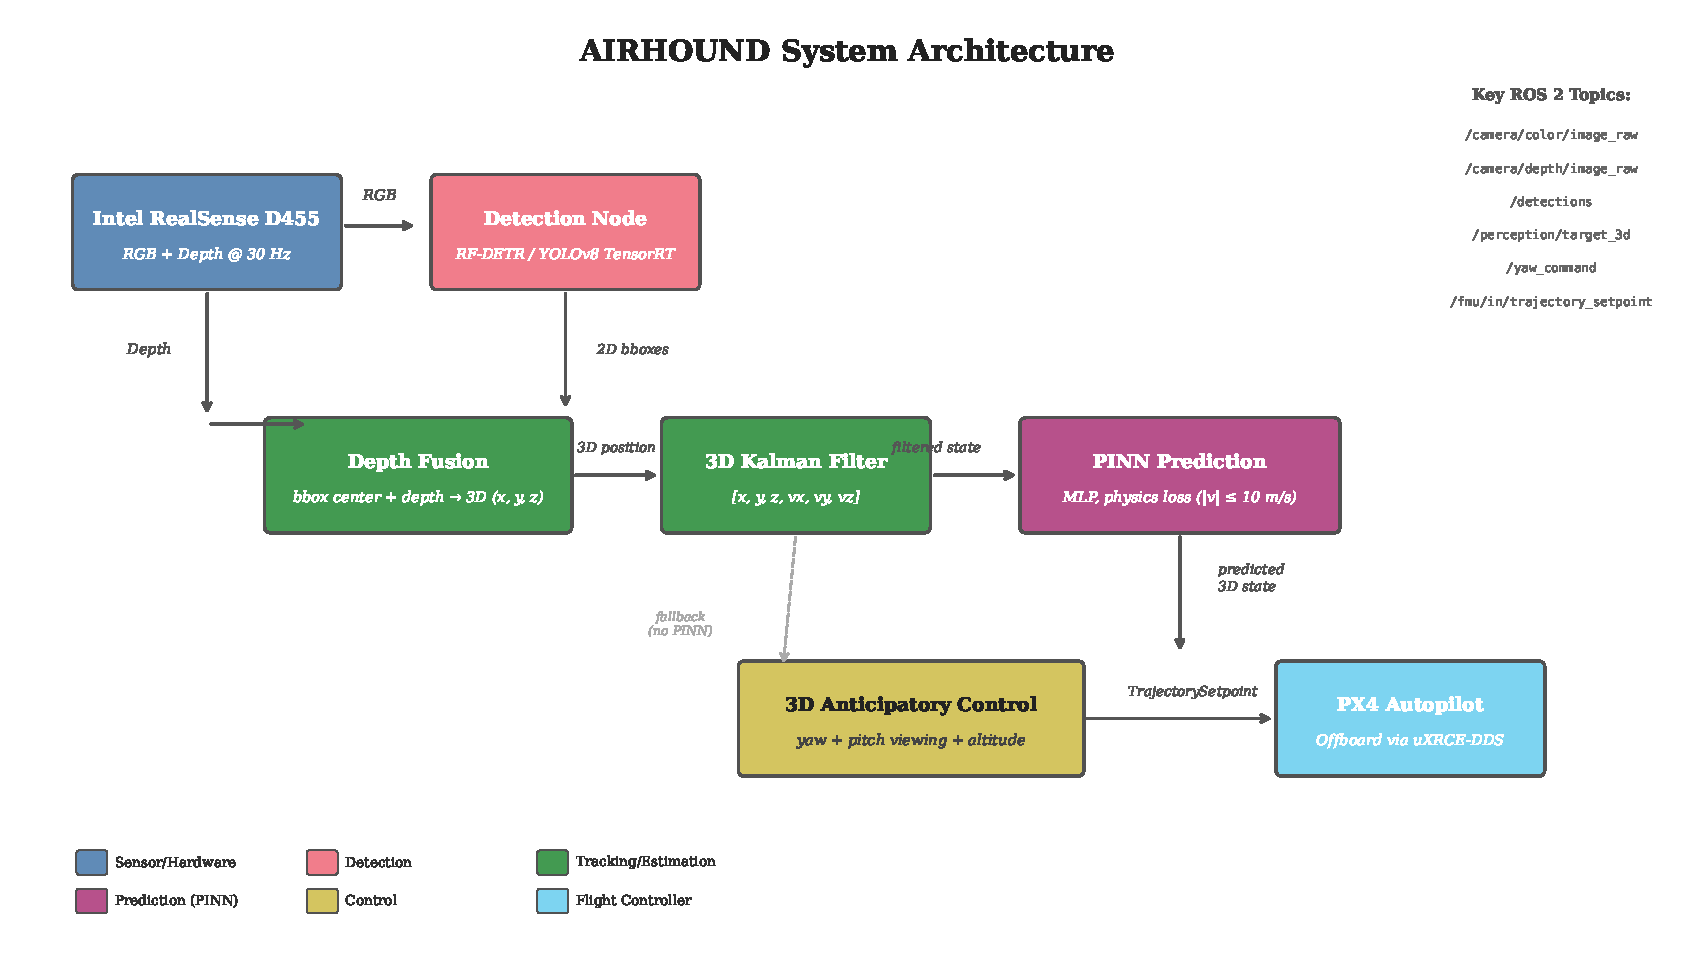
\includegraphics[width=\textwidth]{system_architecture.pdf}
    \caption{AIRHOUND system architecture. The Intel RealSense D455 provides synchronized RGB and depth streams. The detection node (RF-DETR or YOLOv8, selectable via configuration) publishes 2D bounding boxes that are fused with depth to produce 3D position estimates. A 6-state Kalman filter produces smoothed position and velocity, which feeds a PINN for trajectory prediction during detection dropout. The control node commands yaw, pitch viewing angle, and altitude via PX4 offboard mode. A dashed arrow indicates the Kalman-only fallback path when PINN prediction is unavailable.}
    \label{fig:architecture}
\end{figure}

\subsection{Hardware Platform}
\label{sec:hardware}

The UAV platform is a custom quadrotor running PX4~\cite{px4docs} firmware with an NVIDIA Jetson Orin (16~GB) as the companion computer. An Intel RealSense D455~\cite{realsensed455} stereo depth camera provides synchronized RGB ($1280 \times 720$, 30~Hz) and depth ($1280 \times 720$, 30~Hz) streams. The D455's active infrared stereo provides depth measurements in the 0.4--6.0~m range with approximately 1--2\% depth error relative to distance.

Communication between ROS~2 and PX4 is handled by the Micro~XRCE-DDS bridge~\cite{eprosimadds}, which translates between DDS topics and PX4's internal uORB messaging. The bridge runs over UDP on port 8888, enabling the ROS~2 nodes to publish \texttt{TrajectorySetpoint} messages and receive vehicle state at 10~Hz.

\subsection{ROS~2 Pipeline}
\label{sec:ros2_pipeline}

The pipeline consists of five primary nodes:

\begin{enumerate}
    \item \textbf{Detection Node} (\texttt{perception\_node}): Subscribes to \texttt{/camera/color/image\_raw}, runs inference through either the RF-DETR or YOLOv8 TensorRT engine (selected via \texttt{airhound.yaml}), and publishes \texttt{Detection2DArray} messages on \texttt{/detections}. When depth integration is enabled, the node also subscribes to \texttt{/camera/depth/image\_raw}, extracts depth at each bounding box center using a $5 \times 5$ median filter for noise robustness, and embeds the depth value in each detection's pose field.

    \item \textbf{Depth Fusion}: Integrated within the detection node. For each detection, the 2D bounding box center $(u, v)$ and depth $Z$ are projected to 3D camera-frame coordinates using the pinhole camera model: $X = (u - c_x) Z / f_x$, $Y = (v - c_y) Z / f_y$. The highest-confidence detection's 3D position is published on \texttt{/perception/target\_3d} as a \texttt{PointStamped} message.

    \item \textbf{Tracking Node} (\texttt{yaw\_error\_node}): Subscribes to \texttt{/detections}, computes horizontal pixel offset from image center, converts to angular error using camera intrinsics, and publishes yaw rate commands on \texttt{/yaw\_command}. Includes a proportional controller with configurable deadband and rate limits. When detections are absent, the node applies last-rate extrapolation as a short-term prediction.

    \item \textbf{3D Kalman Filter}: A 6-state constant-velocity filter with state vector $\mathbf{x} = [x, y, z, v_x, v_y, v_z]^\top$. The filter uses a standard predict-update cycle with a discrete white noise acceleration process model. Mahalanobis gating rejects outlier measurements (threshold: $\chi^2_{3,0.997} \approx 3.0$), and the filter resets after 30 consecutive missed detections ($\sim$1~s at 30~Hz).

    \item \textbf{Control Node} (\texttt{yaw\_controller\_node}): A C++ node that subscribes to \texttt{/yaw\_command}, constructs PX4 \texttt{TrajectorySetpoint} messages, and streams them at 10~Hz to maintain offboard mode. The current implementation controls yaw only; altitude and pitch viewing extensions are staged for Weeks~5--8 of the development timeline.
\end{enumerate}

\subsection{Model Selection via Configuration}
\label{sec:model_config}

A central configuration file (\texttt{airhound.yaml}) controls detector selection (\texttt{detector\_type}: \texttt{"rfdetr"} or \texttt{"yolo"}), model path, confidence threshold, depth integration parameters, and PX4 control settings. This enables rapid switching between models during comparative flight testing without code changes, ensuring identical test conditions for both detectors.

% ============================================================================
\section{RF-DETR Detection and Degradation Robustness}
\label{sec:rfdetr}

% === THIS IS THE PERCEPTION LEAD'S SECTION ===

\subsection{Model Selection}
\label{sec:model_selection}

We evaluate two object detection architectures for onboard UAV detection: YOLOv8n~\cite{ultralytics2023}, a single-stage CNN-based detector, and RF-DETR~\cite{rfdetr2025}, a transformer-based detection model built on a DINOv2~\cite{oquab2024dinov2} vision encoder with a DETR-style~\cite{carion2020detr} decoder. The selection of these architectures is motivated by the distinct computational paradigms they represent: YOLOv8n processes features through convolutional layers with local receptive fields, while RF-DETR leverages self-attention mechanisms that aggregate global context across the input image.

This architectural distinction has implications for robustness under degraded visual conditions. Convolutional networks rely on local spatial patterns that are directly disrupted by pixel-level noise, low-light conditions, and motion blur. In contrast, the attention mechanism in transformer-based detectors can integrate information from unaffected regions of the image, potentially maintaining detection accuracy when portions of the input are corrupted.

\subsection{Training Configuration}
\label{sec:training}

Both models are trained on a drone detection dataset comprising 13{,}869 training images and 1{,}983 validation images sourced from the Roboflow Drones dataset~\cite{roboflowdrones}, annotated with a single class (\texttt{drone}).

The RF-DETR base variant is used, consisting of a DINOv2 windowed-small encoder with a 3-layer decoder (256 hidden dimension, 300 queries). The model is initialized from COCO-pretrained weights and fine-tuned for 50 epochs with the Adam optimizer (learning rate $1 \times 10^{-4}$, weight decay $1 \times 10^{-4}$), gradient clipping at 0.1 max norm, and 5 warmup epochs. Mixed-precision training (FP16) is used with an effective batch size of 4 on an NVIDIA RTX 4070 (12~GB VRAM). Data augmentation includes mosaic and mixup.

YOLOv8n is trained using the Ultralytics framework with default hyperparameters on the same dataset for a fair comparison.

\subsection{Edge Deployment via TensorRT}
\label{sec:tensorrt}

For real-time inference on the NVIDIA Jetson Orin (16~GB)~\cite{jetsonorin}, both models are converted to TensorRT~\cite{tensorrt} FP16 engines. The RF-DETR conversion pipeline proceeds as:
%
\begin{enumerate}
    \item PyTorch checkpoint $\rightarrow$ ONNX (opset 17, input $560 \times 560$)
    \item ONNX graph simplification via \texttt{onnx-simplifier}
    \item ONNX $\rightarrow$ TensorRT engine via \texttt{trtexec} with FP16 and 4~GB workspace
\end{enumerate}
%
The resulting RF-DETR TensorRT engine is 57~MB and achieves approximately 25~FPS on the Jetson Orin, compared to approximately 1~FPS for the ONNX model on CPU. YOLOv8n TensorRT achieves approximately 30~FPS at $640 \times 640$ input resolution. Both frame rates exceed the 30~Hz camera capture rate, ensuring real-time operation.

\subsection{Synthetic Degradation Pipeline}
\label{sec:degradation_pipeline}

To evaluate robustness under challenging visual conditions---the central theme of the SPIE DS112 track---we apply synthetic degradation to the validation set. Four degradation types are evaluated at five severity levels ($s \in \{0.0, 0.25, 0.5, 0.75, 1.0\}$), where $s = 0.0$ represents the clean baseline:

\begin{itemize}
    \item \textbf{Gaussian noise:} Additive noise with standard deviation $\sigma = s \cdot 50$ (pixel intensity scale 0--255), simulating sensor noise in low-SNR conditions.
    \item \textbf{Low light:} Multiplicative brightness reduction by factor $(1 - 0.9s)$, simulating twilight or shadowed environments.
    \item \textbf{Motion blur:} Directional kernel blur with kernel size $k = \lfloor 20s \rfloor + 1$ pixels, simulating camera or target motion artifacts.
    \item \textbf{Partial occlusion:} Random rectangular patches covering up to $s \cdot 50\%$ of the bounding box area, simulating environmental obstructions.
\end{itemize}

Each degradation is applied independently to all 1{,}983 validation images, yielding $2 \times 4 \times 5 = 40$ unique evaluation conditions (2 models $\times$ 4 degradation types $\times$ 5 severities).

\subsection{Degradation Robustness Results}
\label{sec:degradation_results}

\subsubsection{Clean Baseline}

On clean (undegraded) images, both models achieve comparable performance (Table~\ref{tab:clean_baseline}). YOLOv8n holds a marginal advantage in mAP@0.5 (0.957 vs.\ 0.953) and recall (0.971 vs.\ 0.931), while RF-DETR achieves higher precision (0.949 vs.\ 0.922). This establishes that any performance differences under degradation are attributable to architectural robustness rather than baseline capability gaps.

\begin{table}[htbp]
\centering
\caption{Clean baseline detection performance on 1{,}983 drone images.}
\label{tab:clean_baseline}
\begin{tabular}{lccc}
\hline
\textbf{Metric} & \textbf{YOLOv8n} & \textbf{RF-DETR} & \textbf{$\Delta$} \\
\hline
mAP@0.5 & \textbf{0.957} & 0.953 & -0.005 \\
mAP@0.5:0.95 & \textbf{0.584} & 0.541 & -0.043 \\
Precision & 0.922 & \textbf{0.949} & +0.027 \\
Recall & \textbf{0.971} & 0.931 & -0.040 \\
F1 Score & \textbf{0.946} & 0.940 & -0.006 \\
\hline
\end{tabular}
\end{table}

\subsubsection{Performance Under Degradation}

Figure~\ref{fig:degradation} shows mAP@0.5 as a function of severity level for each degradation type. Two patterns emerge clearly:

\begin{enumerate}
    \item \textbf{Gaussian noise and low light:} RF-DETR maintains significantly higher accuracy as severity increases. At maximum Gaussian noise severity ($s = 1.0$), RF-DETR achieves 0.716 mAP@0.5 compared to YOLOv8n's 0.318---a +39.8 percentage point advantage. Under maximum low-light conditions, the advantage is +39.4 points (0.670 vs.\ 0.275). RF-DETR retains 75\% and 70\% of its clean-baseline performance at maximum noise and low-light severity respectively, while YOLOv8n retains only 33\% and 29\% (Figure~\ref{fig:retention}).

    \item \textbf{Motion blur and occlusion:} Both models are significantly impacted by severe motion blur, with mAP dropping below 0.20 at $s \geq 0.75$. RF-DETR maintains a moderate advantage at low blur severity (+13.9 points at $s = 0.25$), but neither architecture alone can sustain detection at high blur levels. Occlusion performance is comparable, with both models handling partial obstructions gracefully.
\end{enumerate}

\begin{figure}[htbp]
    \centering
    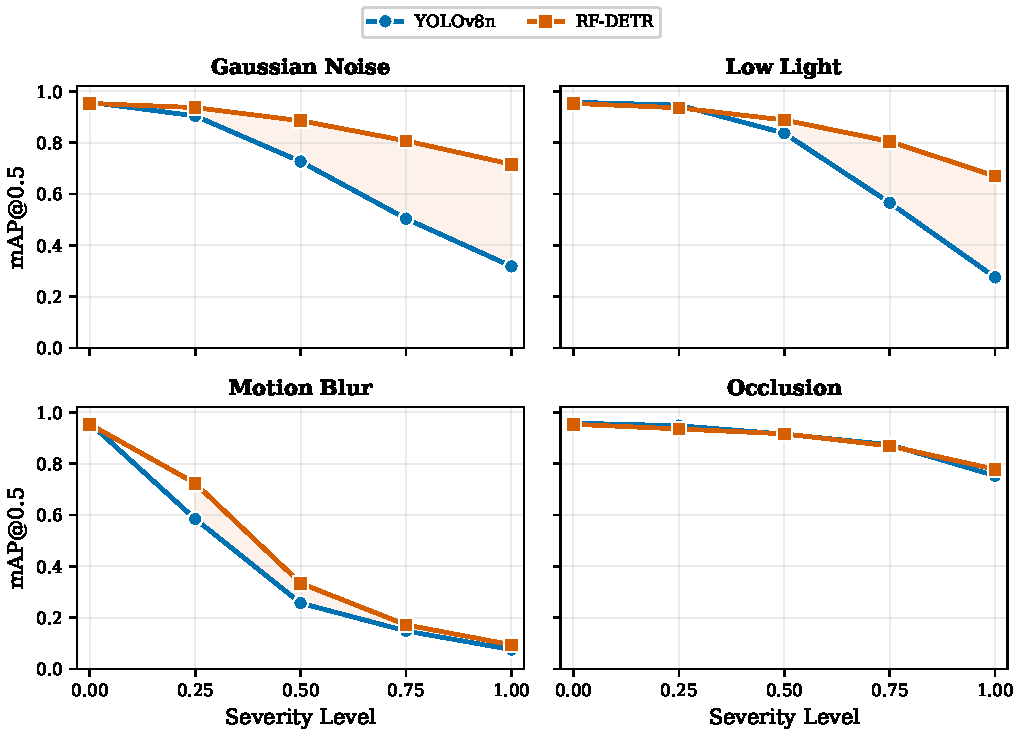
\includegraphics[width=\textwidth]{degradation_comparison.pdf}
    \caption{Detection accuracy (mAP@0.5) under four degradation types at increasing severity. RF-DETR (orange squares) demonstrates substantially higher robustness than YOLOv8n (blue circles) under Gaussian noise and low-light conditions. Shaded region indicates RF-DETR advantage.}
    \label{fig:degradation}
\end{figure}

\begin{figure}[htbp]
    \centering
    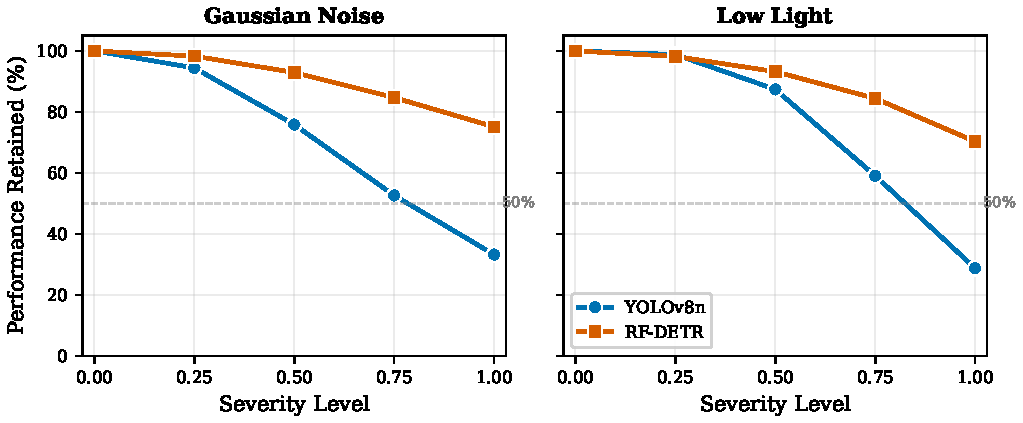
\includegraphics[width=0.85\textwidth]{retention_curve.pdf}
    \caption{Percentage of clean-baseline mAP@0.5 retained under increasing degradation severity for Gaussian noise and low light---the two conditions with the largest architectural performance gap.}
    \label{fig:retention}
\end{figure}

The advantage heatmap (Figure~\ref{fig:heatmap}) provides a complete summary across all conditions. The delta mAP values confirm that RF-DETR's advantage scales with severity: near-zero difference on clean data, growing to $\sim$+0.40 under severe noise and low-light conditions.

\begin{figure}[htbp]
    \centering
    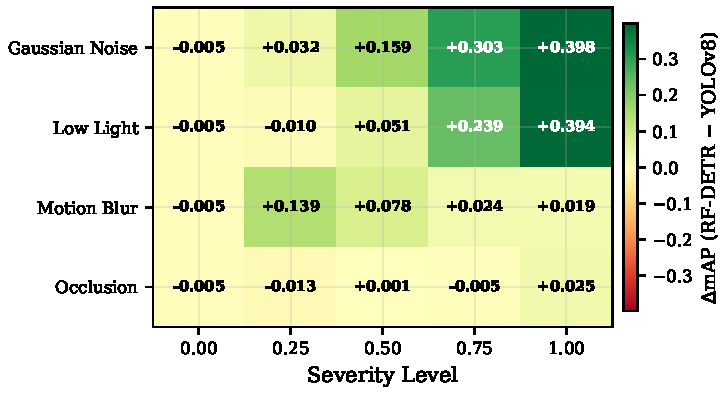
\includegraphics[width=0.75\textwidth]{advantage_heatmap.pdf}
    \caption{Heatmap of mAP@0.5 difference (RF-DETR $-$ YOLOv8n) across all degradation types and severity levels. Green cells indicate RF-DETR outperformance.}
    \label{fig:heatmap}
\end{figure}

Table~\ref{tab:degradation_avg} summarizes the average mAP@0.5 across all severity levels for each degradation type. RF-DETR achieves +17.8 and +13.4 average mAP advantage under Gaussian noise and low light respectively.

\begin{table}[htbp]
\centering
\caption{Average mAP@0.5 across all severity levels (0.0--1.0) by degradation type.}
\label{tab:degradation_avg}
\begin{tabular}{lccc}
\hline
\textbf{Degradation} & \textbf{YOLOv8n} & \textbf{RF-DETR} & \textbf{$\Delta$} \\
\hline
Gaussian Noise & 0.682 & \textbf{0.860} & +0.178 \\
Low Light & 0.716 & \textbf{0.850} & +0.134 \\
Motion Blur & 0.404 & \textbf{0.455} & +0.051 \\
Occlusion & 0.889 & \textbf{0.890} & +0.001 \\
\hline
\end{tabular}
\end{table}

\subsubsection{Implications for System Design}

These results inform two key architectural decisions:

\begin{enumerate}
    \item \textbf{Detector selection:} RF-DETR is selected as the primary detector for flight operations. Its robustness advantage under noise and lighting variation---conditions frequently encountered in outdoor UAV operations---outweighs YOLOv8n's marginal clean-data and speed advantages. Both models are retained in the pipeline, switchable via configuration, to enable comparative flight testing.

    \item \textbf{Complementary prediction:} The severe performance degradation of both models under motion blur ($<$0.20 mAP at $s \geq 0.75$) motivates the integration of a predictive tracking component. Detection dropouts during blur events must be bridged by Kalman filtering and PINN-based trajectory prediction (Sections~\ref{sec:depth} and~\ref{sec:pinn}).
\end{enumerate}

% ============================================================================
\section{Depth Integration and 3D State Estimation}
\label{sec:depth}

Monocular object detection alone provides only 2D image-plane localization. To enable 3D control (altitude hold, pitch viewing), the system fuses 2D detections with stereo depth from the RealSense D455.

\subsection{Depth Extraction and Filtering}
\label{sec:depth_extraction}

For each detection bounding box, the system extracts depth at the box center pixel $(u_c, v_c)$. To mitigate stereo matching noise---particularly at object edges and at ranges beyond 3~m---a $5 \times 5$ median filter is applied over a window centered on $(u_c, v_c)$. Only depth values within the D455's reliable operating range (0.4--6.0~m) are accepted; values outside this range are flagged as invalid and downstream consumers receive \texttt{NaN}.

The D455 publishes 16-bit unsigned depth images in millimeters. A configurable scale factor ($\alpha = 0.001$) converts to meters:
\begin{equation}
    Z = \alpha \cdot \text{median}\left(\mathbf{D}[v_c \pm 2, u_c \pm 2]\right)
    \label{eq:depth}
\end{equation}
where $\mathbf{D}$ is the depth image and the window excludes zero-valued (invalid) pixels before computing the median.

\subsection{3D Projection}
\label{sec:projection}

Given a valid depth $Z$ and camera intrinsics $(f_x, f_y, c_x, c_y)$ from the \texttt{CameraInfo} topic, the 3D position in the camera optical frame is computed using the pinhole model:
\begin{equation}
    X = \frac{(u_c - c_x) \cdot Z}{f_x}, \quad
    Y = \frac{(v_c - c_y) \cdot Z}{f_y}, \quad
    Z = Z
    \label{eq:projection}
\end{equation}
The resulting $(X, Y, Z)$ is published as a \texttt{PointStamped} message on \texttt{/perception/target\_3d} in the \texttt{camera\_color\_optical\_frame} coordinate frame, where $+X$ is right, $+Y$ is down, and $+Z$ is forward (into the scene).

\subsection{3D Kalman Filter}
\label{sec:kalman}

A 6-state constant-velocity Kalman filter~\cite{kalmanfilter1960} estimates the target's 3D position and velocity from noisy depth-fused measurements. The state vector is:
\begin{equation}
    \mathbf{x} = [x, y, z, v_x, v_y, v_z]^\top
\end{equation}

\subsubsection{Motion Model}

The state transition follows a constant-velocity assumption:
\begin{equation}
    \mathbf{x}_{k+1} = \mathbf{F}(\Delta t) \, \mathbf{x}_k + \mathbf{w}_k, \quad
    \mathbf{F} = \begin{bmatrix}
        \mathbf{I}_3 & \Delta t \, \mathbf{I}_3 \\
        \mathbf{0}_3 & \mathbf{I}_3
    \end{bmatrix}
\end{equation}
where $\Delta t$ is the inter-frame interval and $\mathbf{w}_k \sim \mathcal{N}(\mathbf{0}, \mathbf{Q})$ is the process noise. The process noise covariance uses a diagonal model with separate position and velocity noise terms, tuned based on expected target maneuverability.

\subsubsection{Measurement Model}

The measurement vector $\mathbf{z}_k = [x, y, z]^\top$ is the 3D position from depth fusion. The observation matrix $\mathbf{H} = [\mathbf{I}_3 \;\; \mathbf{0}_3]$ selects the position components. The measurement noise covariance $\mathbf{R}$ is set based on D455 depth accuracy characteristics: approximately $\sigma_z \approx 0.01 Z$ for the depth axis and $\sigma_{x,y} \approx Z / f$ for the lateral axes, where $f$ is the focal length in pixels.

\subsubsection{Update and Gating}

The filter uses the Joseph-form covariance update for numerical stability:
\begin{equation}
    \mathbf{P}_{k|k} = (\mathbf{I} - \mathbf{K}_k \mathbf{H}) \, \mathbf{P}_{k|k-1} \, (\mathbf{I} - \mathbf{K}_k \mathbf{H})^\top + \mathbf{K}_k \mathbf{R} \mathbf{K}_k^\top
\end{equation}

Outlier measurements are rejected using a Mahalanobis distance gate:
\begin{equation}
    d_M = \sqrt{(\mathbf{z}_k - \mathbf{H}\hat{\mathbf{x}}_{k|k-1})^\top \mathbf{S}_k^{-1} (\mathbf{z}_k - \mathbf{H}\hat{\mathbf{x}}_{k|k-1})}
\end{equation}
where $\mathbf{S}_k = \mathbf{H} \mathbf{P}_{k|k-1} \mathbf{H}^\top + \mathbf{R}$ is the innovation covariance. Measurements with $d_M > 3.0$ are rejected ($\sim$99.7\% confidence for 3~DOF). After 30 consecutive rejected or missing measurements ($\sim$1~s at 30~Hz), the filter resets and reinitializes on the next valid detection.

\subsection{Depth Quality Monitoring}
\label{sec:depth_quality}

The perception node publishes real-time depth quality metrics: a binary availability flag on \texttt{/perception/depth\_available} and a per-frame quality ratio (valid depths / total detections) on \texttt{/perception/depth\_quality}. These enable downstream nodes to adapt behavior when depth is unreliable---for example, falling back to 2D-only tracking when depth quality drops below a configurable threshold.

% ============================================================================
\section{Physics-Informed Trajectory Prediction}
\label{sec:pinn}
% TODO: Tracking team
% - PINN architecture (MLP, input/output spec)
% - Physics loss function (velocity constraint)
% - Training pipeline (SITL + real data)
% - Dropout recovery mechanism
% - Online update proof-of-concept (if applicable)

% ============================================================================
\section{Anticipatory Control}
\label{sec:control}
% TODO: Controls (primary), Tracking team contributes
% - 3D control node: yaw + pitch viewing + altitude
% - PID structure for each axis
% - Safety limits and failsafe behavior
% - PINN-driven anticipatory commands during dropout

% ============================================================================
\section{Experimental Setup}
\label{sec:experiments}

Evaluation proceeds in two stages: software-in-the-loop (SITL) simulation for system integration validation, followed by hardware flight testing for real-world performance characterization.

\subsection{SITL Validation}
\label{sec:sitl}

SITL testing uses PX4's Gazebo~\cite{gazebo2004} integration with a simulated X500 quadrotor. A mock detector generates synthetic detection sequences with configurable target motion patterns (circular, sinusoidal, figure-eight, and static), publish rate, bounding box size, and optional Gaussian noise. This enables end-to-end pipeline testing---from detection through Kalman filtering, prediction, and control---without requiring camera hardware.

The SITL environment serves three purposes:
\begin{enumerate}
    \item \textbf{Integration testing}: Verifying that all ROS~2 nodes communicate correctly, PX4 enters and maintains offboard mode, and the control loop is stable.
    \item \textbf{PINN training data}: Scripted target motion scenarios (10+, including vertical motion for altitude control validation) generate rosbag recordings of 3D position trajectories used to train the PINN (Section~\ref{sec:pinn}).
    \item \textbf{Control tuning}: Initial PID parameter tuning for yaw, pitch, and altitude axes before transferring to hardware.
\end{enumerate}

% TODO: Add SITL results after completing integration tests

\subsection{Hardware Flight Testing}
\label{sec:flight_testing}

Hardware flights are conducted in an indoor flight cage at Embry-Riddle Aeronautical University using a static or hand-held target. The flight test matrix evaluates both detectors under controlled scenarios:

\begin{table}[htbp]
    \centering
    \caption{Flight test matrix. Each scenario is tested with both YOLOv8 and RF-DETR detectors.}
    \label{tab:flight_matrix}
    \begin{tabular}{lll}
        \toprule
        \textbf{Scenario} & \textbf{Motion Type} & \textbf{Primary Test} \\
        \midrule
        Steady hover     & Static target         & Baseline stability \\
        Slow linear      & Horizontal, $<$1 m/s  & Yaw tracking \\
        Moderate speed   & Horizontal, 1--2 m/s  & Yaw tracking \\
        Vertical motion  & Up/down               & Pitch viewing \\
        Approach/retreat & Toward/away            & Altitude control \\
        Diagonal 3D      & Combined axes          & Full 3D control \\
        Natural occlusion & Partial obstruction   & Dropout recovery \\
        Varying distance  & 1--5 m range          & Depth accuracy \\
        \bottomrule
    \end{tabular}
\end{table}

\subsection{Data Collection}
\label{sec:data_collection}

Each flight records a ROS~2 rosbag containing:
\begin{itemize}
    \item \texttt{/detections}: Detection2DArray with embedded depth
    \item \texttt{/camera/camera\_info}: Camera intrinsics
    \item \texttt{/target\_yaw}: Computed yaw commands
    \item \texttt{/fmu/in/trajectory\_setpoint}: Control commands sent to PX4
    \item \texttt{/fmu/in/offboard\_control\_mode}: Offboard mode status
    \item \texttt{/fmu/in/vehicle\_command}: Arming and mode commands
\end{itemize}
PX4 flight logs are downloaded separately for ground-truth attitude and position data. Environmental conditions (lighting, temperature) are logged per flight.

\subsection{Evaluation Metrics}
\label{sec:metrics}

The following metrics are computed from flight data:
\begin{itemize}
    \item \textbf{Detection}: mAP@0.5, precision, recall, inference latency, and FPS for each detector.
    \item \textbf{Tracking}: Detection dropout duration, recovery time (frames from dropout to re-acquisition), and 3D position estimation error relative to ground truth.
    \item \textbf{Prediction}: PINN vs.\ Kalman extrapolation comparison using RMSE and maximum position error during dropout intervals.
    \item \textbf{Control}: Yaw tracking error (degrees), altitude maintenance accuracy (meters), and response time to step changes in target position.
\end{itemize}

% TODO: Populate with actual flight data results

% ============================================================================
\section{Results}
\label{sec:results}
% TODO: Lead (primary), all contribute data
% - Detection comparison (flight data)
% - Tracking accuracy (dropout duration, recovery time)
% - PINN vs Kalman prediction comparison
% - Control performance (yaw, pitch, altitude error)
% - Combined system performance

% ============================================================================
\section{Discussion}
\label{sec:discussion}
% TODO: Lead
% - Key findings synthesis
% - Limitations
% - Comparison with prior work

% ============================================================================
\section{Conclusion}
\label{sec:conclusion}
% TODO: Lead
% - Summary of contributions
% - Future work (full autonomy, multi-target, etc.)

% ============================================================================
\section*{Acknowledgments}
% Faculty advisor: Dr. Drakunov
% EPPL Lab, Embry-Riddle Aeronautical University
% SPIE Student Conference Support (if awarded)

% ============================================================================
\bibliographystyle{unsrtnat}
\bibliography{references}

\end{document}
